\documentclass{beamer}
\usepackage{graphics}
\usepackage{epsfig}
\usepackage{multicol}
\usepackage{pifont}
\setbeamertemplate{navigation symbols}{}
\newcommand{\RR}{\ensuremath{\mathbb{R}}}
\newcommand{\NN}{\ensuremath{\mathbb{N}}}
\newcommand{\QQ}{\ensuremath{\mathbb{Q}}}
\newcommand{\CC}{\ensuremath{\mathbb{C}}}
\newcommand{\ZZ}{\ensuremath{\mathbb{Z}}}
\newcommand{\TT}{\ensuremath{\mathbb{T}}}
\DeclareMathOperator{\Min}{Min}
\DeclareMathOperator{\Dom}{Dom}
\DeclareMathOperator{\vol}{vol}
\DeclareMathOperator{\Aut}{Aut}
\DeclareMathOperator{\Stab}{Stab}
\DeclareMathOperator{\Sym}{Sym}
\DeclareMathOperator{\Grp}{Grp}
\DeclareMathOperator{\GL}{GL}
\DeclareMathOperator{\Id}{Id}

\begin{document}
\title{My works with Michel Deza on Polytopes and related structures}
\author{
{\small
\begin{center}
\textcolor{red}{\large Mathieu Dutour Sikiri\'c}\\[2mm]
\textcolor{red}{Institut Rudjer Bo\u skovi\'c, Zagreb}
%\textcolor{red}{Institut Rudjer Bo\u skovi\'c, Zagreb, Institute of Statistical Mathematics and Hayama}
\end{center}
}
}
\date{\today}

\frame{\titlepage}


\frame{
\begin{center}
\begin{tabular*}{7cm}{c}
\\[-0.5cm]
{\Huge
\textcolor{blue}{I. }\textcolor{red}{Hypermetrics}
}
\end{tabular*}
\end{center}
}


\frame{
  \frametitle{Hypermetric inequalities and cones}

\begin{itemize}
\item We consider metrics on $n$ points, defined by a function $(d_{i,j})_{1\leq i,j\leq n}$
\item Given a vector $v\in \ZZ^n$ with $\sum_i b_i = 1$ the hypermetric inequality is
  \begin{equation*}
  \sum_{1\leq i<j\leq n} b_i b_j d_{i,j}\leq 0
  \end{equation*}
\item The hypermetric cone $HYP_{n}$ is defined as the set of functions $(d_{i,j}$ satifying to 
\end{itemize}

}







\frame{
\begin{center}
\begin{tabular*}{7cm}{c}
\\[-0.5cm]
{\Huge
\textcolor{blue}{II. }\textcolor{red}{Space fullerenes}
}
\end{tabular*}
\end{center}
}





\frame{
  \frametitle{Frank Kasper structures}

\begin{itemize}
\item There are exactly $4$ fullerenes with isolated hexagons:
\begin{center}
\begin{minipage}[b]{24mm}
\centering
\epsfig{height=18mm, file=SpaceFullPicture/F1-crop.pdf}\par
%\resizebox{18mm}{!}{\rotatebox{90}{\includegraphics[bb=86 165 524 626,clip]{SpaceFullPicture/F1.pdf}}}\par
20, $I_h$
\end{minipage}
\begin{minipage}[b]{24mm}
\centering
\epsfig{height=18mm, file=PictureAppli/F2sec-crop.pdf}\par
%\resizebox{20mm}{!}{\includegraphics[bb=1 1 440 381, clip]{PictureAppli/F2sec.pdf}}\par
%\resizebox{18mm}{!}{\rotatebox{0}{\includegraphics[bb=86 206 524 590,clip]{SpaceFullPicture/F2.pdf}}}\par
24 $D_{6d}$
\end{minipage}
\begin{minipage}[b]{24mm}
  \centering
\epsfig{height=18mm, file=FullPresPic/Picture2-crop.pdf}\par
%\resizebox{20mm}{!}{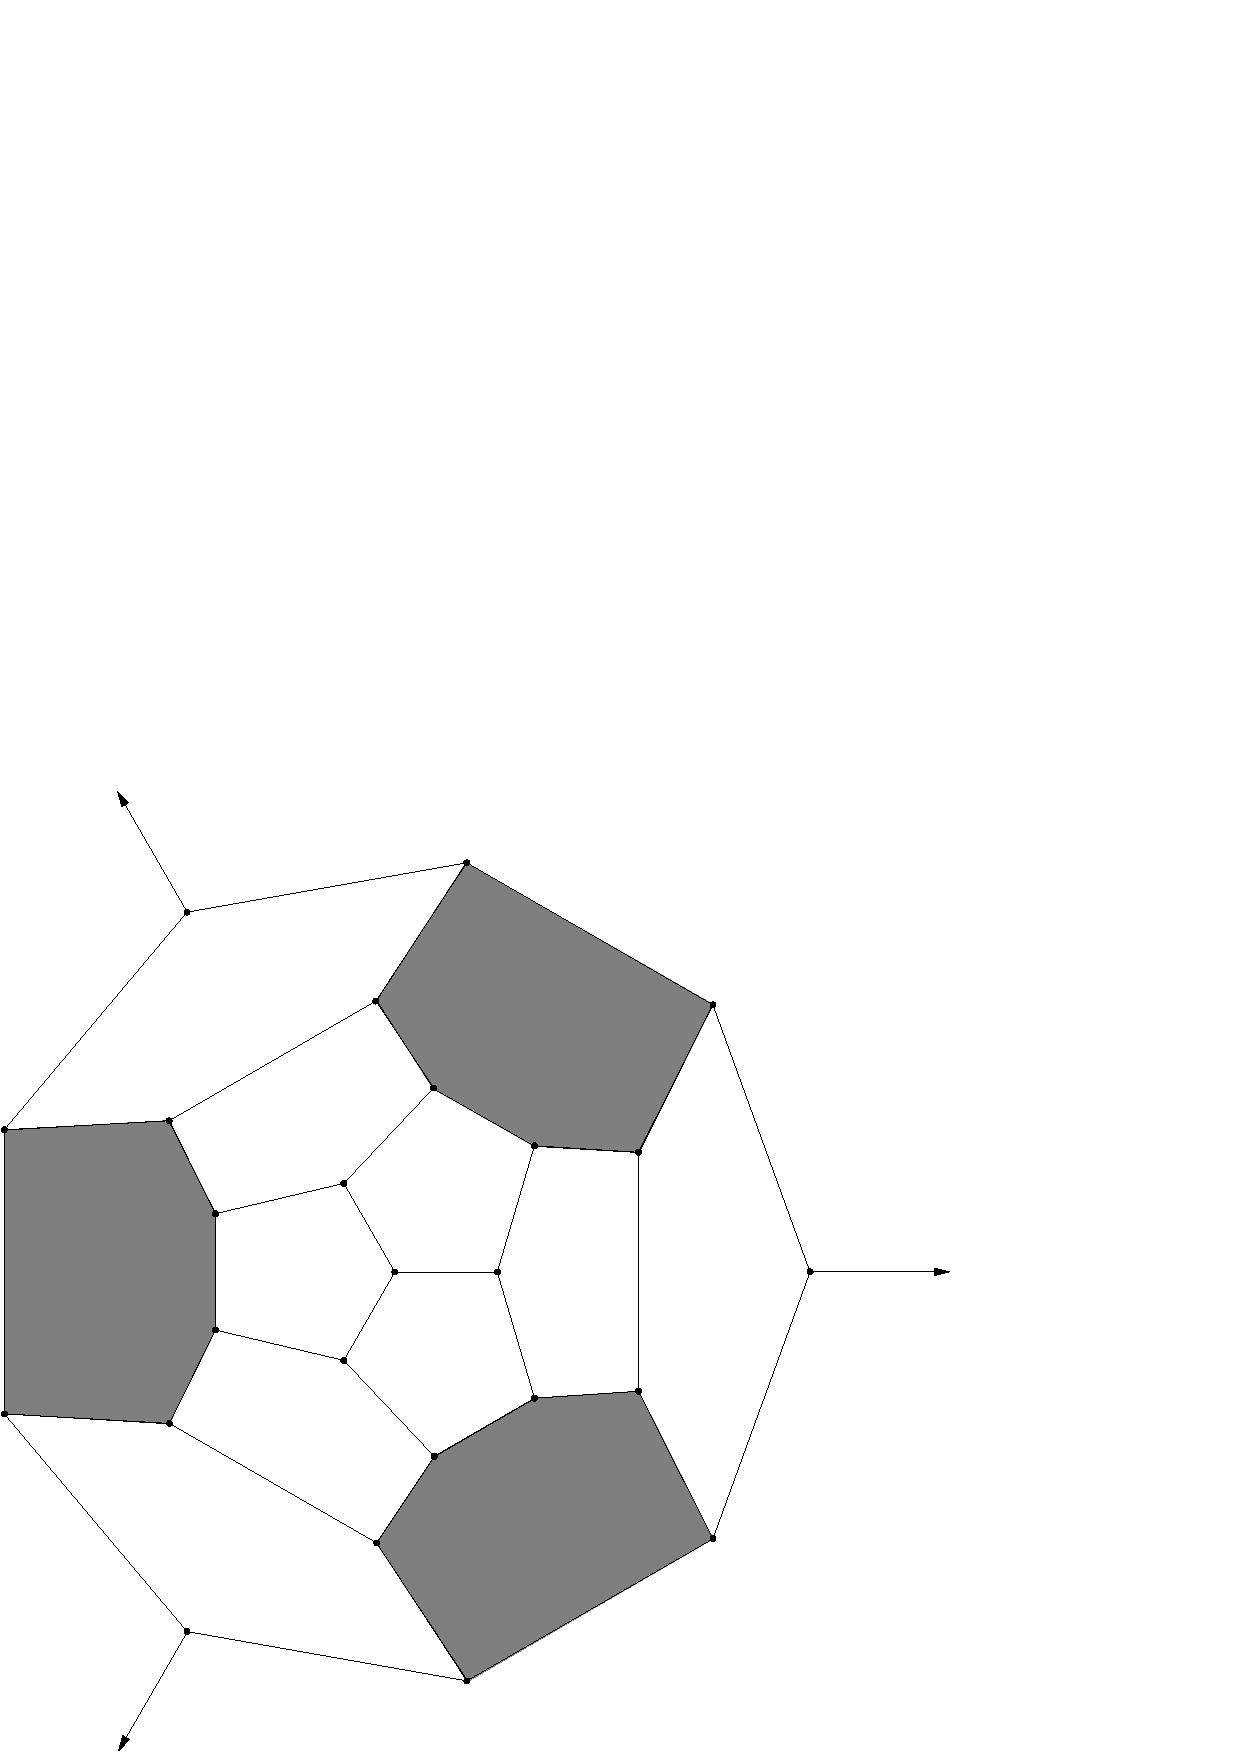
\includegraphics[bb=1 1 457 464, clip]{FullPresPic/Picture2.pdf}}\par
%\resizebox{18mm}{!}{\rotatebox{0}{\includegraphics[bb=86 206 524 590,clip]{SpaceFullPicture/F3.pdf}}}\par
26, $D_{3h}$
\end{minipage}
\begin{minipage}[b]{24mm}
  \centering
\epsfig{height=18mm, file=PictureAppli/F4sec-crop.pdf}\par
%\resizebox{20mm}{!}{\includegraphics[bb=1 1 439 380, clip]{PictureAppli/F4sec.pdf}}\par
%\resizebox{18mm}{!}{\rotatebox{0}{\includegraphics[bb=86 206 524 590,clip]{SpaceFullPicture/F4.pdf}}}\par
28, $T_{d}$
\end{minipage}
\end{center}
\item A \textcolor{red}{Space-fullerene} structure is a $4$-valent $3$-periodic tiling of $\RR^3$ by those $4$ fullerenes.
\item They were introduced by Frank \& Kasper in two papers in 1958, 1959 in order to explain a variety of crystallographic structures in a unified way.
\item The basic problems are:
\begin{itemize}
\item Find the possible structures, they are very rare.
\item Find some general constructions.
\item Find structural properties.
\end{itemize}

\end{itemize}
}


\frame{
  \frametitle{Known Physical phases I}

\begin{itemize}
\item \textcolor{red}{group} is the space group according to the crystallographic tables
\item \textcolor{red}{fund. dom.} is the number of cells in a fundamental domain.
\item \textcolor{red}{fraction} $(x_{20}, x_{24}, x_{26}, x_{28})$ is the relative number of $20$-, $24$-, $26$- and $28$-cells in 
\end{itemize}
\begin{center}
{\small
\begin{tabular}{|c|c|c|c|c|}
\cline{1-5}
phase & rep. alloy & group & fund. dom. & fraction\\
\cline{1-5}
$C_{14}$ & ${\rm Mg} {\rm Zn}_{2}$ & $P6_3/mmc$ & $12$ & $(2,0,0,1)$\\
$C_{15}$ & ${\rm Mg} {\rm Cu}_{2}$ & $Fd\overline{3}m$ & $24$ & $(2,0,0,1)$\\
$C_{36}$ & ${\rm Mg} {\rm Ni}_{2}$ & $P6_3/mmc$ & $24$ &  $(2,0,0,1)$\\
$6$-layers & ${\rm Mg} {\rm Cu} {\rm Ni}$ & $P6_3/mmc$ & $36$ &  $(2,0,0,1)$\\
$8$-layers & ${\rm Mg} {\rm Zn}_2 + 0.03 {\rm Mg} {\rm Ag}_2$ & $P6_3/mmc$ & $48$ & $(2,0,0,1)$\\
$9$-layers & ${\rm Mg} {\rm Zn}_2 + 0.07 {\rm Mg} {\rm Ag}_2$ & $R\overline{3}m$ & $54$ & $(2,0,0,1)$\\
$10$-layers & ${\rm Mg} {\rm Zn}_2 + 0.1 {\rm Mg} {\rm Ag}_2$ & $P6_3/mmc$ & $60$ & $(2,0,0,1)$\\
$-$ & ${\rm Mg}_4{\rm Zn}_7$ & $C2/m$ & $110$ & $(35,2,2,16)$\\
$X$ & ${\rm Mn}_{45} {\rm Co}_{40} {\rm Si}_{15}$ & $Pnnm$ & $74$ & $(23,2,2,10)$\\
$T$ & ${\rm Mg}_{32}(Zn, Al)_{49}$ & $Im\overline{3}$ & $162$ & $(49,6,6,20)$\\
$C$ & ${\rm V}_{2} ({\rm Co}, {\rm Si})_{3}$ & $C2/m$ & $50$ & $(15,2,2,6)$\\
\cline{1-5}
\end{tabular}
}
\end{center}

}


\frame{
  \frametitle{Known Physical phases II}


\begin{center}
{\small
\begin{tabular}{|c|c|c|c|c|}
\cline{1-5}
phase & rep. alloy & group & fund. dom. & fraction\\
\cline{1-5}
$-^{\star}$ & ${\rm K}_{7} {\rm Cs}_{6}$ & $P6_3/mmc$ & $26$ & $(7,2,2,2)$\\
$p\sigma$ & ${\rm Th}_{6} {\rm Cd}_{7}$ & $Pbam$ & $26$ & $(7,2,2,2)$\\
$\mu$ & ${\rm Mo}_{6} {\rm Co}_{7}$ & $R\overline{3}m$ & $39$ & $(7,2,2,2)$\\
$M$ & ${\rm Nb}_{48} {\rm Ni}_{39} {\rm Al}_{13}$ & $Pnma$ & $52$ & $(7,2,2,2)$\\
$R$ & ${\rm Mo}_{31} {\rm Co}_{51} {\rm Cr}_{18}$ & $R\overline{3}$ & $159$ & $(27,12,6,8)$\\
$K^{\star}$ & ${\rm Mn}_{77} {\rm Fe}_{4} {\rm Si}_{19}$ & $C2$ & $110$ & $(25,19,4,7)$\\
$Z$ & ${\rm Zr}_{4} {\rm Al}_{3}$ & $P6/mmm$ & $7$ & $(3,2,2,0)$\\
$P$ & ${\rm Mo}_{42} {\rm Cr}_{18} {\rm Ni}_{40}$ & $Pnma$ & $56$ & $(6,5,2,1)$\\
$\delta$ & ${\rm Mo} {\rm Ni}$ & $P2_12_12_1$ & $56$ & $(6,5,2,1)$\\
$\nu$ & ${\rm Mn}_{81.5} {\rm Si}_{18.5}$ & $Immm$ & $186$ & $(37,40,10,6)$\\
$J$ & complex & $Pmmm$ & $22$ & $(4,5,2,0)$\\
$F$ & complex & $P6/mmm$ & $52$ & $(9,13,4,0)$\\
$K$ & complex & $Pmmm$ & $82$ & $(14,21,6,0)$\\
$H$ & complex & $Cmmm$ & $30$ & $(5,8,2,0)$\\
$\sigma$ & ${\rm Cr}_{46} {\rm Fe}_{54}$ & $P4_2/mnm$ & $30$ & $(5,8,2,0)$\\
$A_{15}$ & ${\rm Cr}_{3} {\rm Si}$ & $Pm\overline{3}n$ & $8$ & $(1,3,0,0)$\\
\cline{1-5}
\end{tabular}
}
\end{center}

}








\frame{
  \frametitle{Enumeration results}
\begin{itemize}
\item We enumerate periodic structures having a fundamental domain containing at most $N$ maximal cells.
\item Note that the cells are not all congruent, Dodecahedron is not necessarily regular and the faces of ``polytopes'' can be curved.
\item For every structure, we have a fractional formula $(x_{20}, x_{24}, x_{26}, x_{28})$.
\item For $N=20$, we get $84$ structures in $1$ month of computations on about $200$ processors.
Going from $N$ to $N+1$, computation time multiply by around $2.3$.
\end{itemize}

{\scriptsize
\begin{center}
\begin{tabular}{||c|c||c|c||c|c||}
\hline
$(1,3,0,0)$ & $1$ & $(2,0,0,1)$ & $5$ & $(3,2,2,0)$ & $4$\\
$(3,3,0,1)$ & $3$ & $(3,3,2,0)$ & $1$ & $(3,4,2,0)$ & $3$\\
$(4,5,2,0)$ & $1$ & $(5,2,2,1)$ & $20$ & $(5,3,0,2)$ & $3$\\
$(5,8,2,0)$ & $2$ & $(6,5,2,1)$ & $6$ & $(6,11,2,0)$ & $1$\\
$(7,2,2,2)$ & $5$ & $(7,4,2,2)$ & $1$ & $(7,7,4,0)$ & $1$\\
$(7,8,2,1)$ & $1$ & $(8,4,4,1)$ & $2$ & $(8,5,2,2)$ & $2$\\
$(9,2,2,3)$ & $1$ & $(10,3,6,1)$ & $3$ & $(10,5,2,3)$ & $6$\\
$(11,1,4,3)$ & $1$ & $(11,2,2,4)$ & $11$ & &\\
\hline
\end{tabular}
\end{center}
}
}







\frame{
  \frametitle{Other structure $(3,2,2,0)$}

\begin{center}
\resizebox{9.5cm}{!}{\includegraphics{SpaceFullPicture/Struct14_63.pdf}}\par
\end{center}
}
\frame{
  \frametitle{Other structure $(3,2,2,0)$}

\begin{center}
\resizebox{9.5cm}{!}{\includegraphics{SpaceFullPicture/Struct14_65.pdf}}\par
\end{center}
}
\frame{
  \frametitle{Other structure $(3,2,2,0)$}

\begin{center}
\resizebox{9.5cm}{!}{\includegraphics{SpaceFullPicture/Struct14_78.pdf}}\par
\end{center}
}







\frame{
  \frametitle{One structure $(3,3,0,1)$}

\begin{center}
\resizebox{9.5cm}{!}{\includegraphics{SpaceFullPicture/Struct14_52.pdf}}\par
\end{center}
}
\frame{
  \frametitle{One structure $(3,3,0,1)$}
\begin{center}
\resizebox{9.5cm}{!}{\includegraphics{SpaceFullPicture/Struct14_54.pdf}}\par
\end{center}
}
\frame{
  \frametitle{One structure $(3,3,0,1)$}

\begin{center}
\resizebox{9.5cm}{!}{\includegraphics{SpaceFullPicture/Struct14_74.pdf}}\par
\end{center}
}








\frame{
  \frametitle{One structure $(7,2,2,2)$}

\begin{center}
\resizebox{9.5cm}{!}{\includegraphics{SpaceFullPicture/Struct39.pdf}}\par
\end{center}
It is a mix of $C_{15}$ and $A_{15}$ in layers.
}



\frame{
  \frametitle{One structure $(7,2,2,2)$}

\begin{center}
\resizebox{9.5cm}{!}{\includegraphics{SpaceFullPicture/Struct41.pdf}}\par
\end{center}
It is a mix of $Z$ and $C_{15}$ in layers.
}

\frame{
  \frametitle{One structure $(5,2,2,1)$}

\begin{center}
\resizebox{9.5cm}{!}{\includegraphics{SpaceFullPicture/Struct18.pdf}}\par
\end{center}
%It is a mix of $Z$ and $C_{15}$ in layers.
}





\frame{
  \frametitle{One structure $(4,5,2,0)$}

\begin{center}
\resizebox{9.5cm}{!}{\includegraphics{SpaceFullPicture/Struct19.pdf}}\par
\end{center}
It is a mix of $Z$ and $A_{15}$ in layers.
}











\frame{
  \frametitle{Yarmolyuk Kripyakevich conjecture}

\begin{itemize}
\item They conjectured that for a space fullerene to exist, we should have 
\begin{equation*}
-x_{20}+\frac{x_{24}}{3}+\frac{7}{6}x_{26}+2x_{28} = 0
\end{equation*}
\item But some counterexamples were found:
\begin{center}
\epsfig{width=7.5cm, file=SpaceFullPicture/Struct14_17-crop.pdf}\par
%\resizebox{7.5cm}{!}{\includegraphics[bb=20 47 752 498, clip]{SpaceFullPicture/Struct14_17.pdf}}\par
\end{center}
\item Some other conjecture are broken.

\end{itemize}
}




\frame{
\begin{center}
\begin{tabular*}{7cm}{c}
\\[-0.5cm]
{\Huge
\textcolor{blue}{III. }\textcolor{red}{Zigzags and central circuits}
}
\end{tabular*}
\end{center}
}




\frame{
\begin{center}
\begin{tabular*}{7cm}{c}
\\[-0.5cm]
{\Huge
\textcolor{blue}{IV. }\textcolor{red}{Elliptic polycycles}
}
\end{tabular*}
\end{center}
}






\end{document}
